% ------------------------------------------------------------------------------
% Este fichero es parte de la plantilla LaTeX para la realización de Proyectos
% Final de Grado, protegido bajo los términos de la licencia GFDL.
% Para más información, la licencia completa viene incluida en el
% fichero fdl-1.3.tex

% Copyright (C) 2012 SPI-FM. Universidad de Cádiz
% ------------------------------------------------------------------------------
\begin{comment}
A continuación, se describe la motivación del presente proyecto y su alcance. También se incluye un glosario de términos y la organización del resto de la presente documentación.
\end{comment}

\label{chapter:introduccinon}

El presente \pfc{} ha sido desarrollado en el \gls{dlr} contando con el apoyo del \gls{scvss}, el \gls{vf} y el \gls{fw} y la supervisión de mi tutor \profname{} durante todo el proceso de desarrollo.

% \section{El Centro Aeroespacial Alemán (DLR)}
\label{section:dlr}

\begin{wrapfigure}{r}{0.3\textwidth}
  \begin{center}
    
\includegraphics[width=0.29\textwidth]{dlr-logo.jpg}
  \end{center}
  \caption{Logotipo \gls{dlr}}
\end{wrapfigure}

El \gls{dlr} es una de las instituciones públicas más importantes dedicadas a la investigación en la República Federal Alemana.\\ 

Sus oficinas centrales se encuentran en la ciudad de Colonia, más de 15 delegaciones, con 32 institutos, repartidas por el territorio nacional alemán y 5 situadas a lo largo del mundo \cite{dlrort}. Actualmente cuenta con más de 7.700 trabajadores y un presupuesto anual dependiente del \gls{bmwi}- de 157 millones de euros para el año 2014 \cite{haushalt2014}.\\


En instituciones orientadas a la investigación, como es el \gls{dlr}, la gestión del conocimiento tiene un significado muy importante. Dado el cambio de personal constante involucrado en las distintas fuentes de conocimiento, reside el peligro de pérdida del mismo. \\

La importancia de la gestión del conocimiento es debido a que éste concreta las actividades de una entidad. Estas actividades ``tienen como meta una mejora de la gestión específica de la organización tanto para el conocimiento interno como externo'' \cite{cissek}. Por lo tanto, el objetivo no debería de ser sólo el almacenamiento sino también la recuperación y reutilización del conocimiento obtenido en situaciones anteriores \cite{dengel}.\\


\subsection{``Transporte y la Movilidad'' en el DLR}

Junto con materias relacionadas con la aeronáutica, el espacio, la energía y la seguridad, el transporte es uno de sus temas de estudio, destacando la evolución de éste como unos de los puntos de trabajo más importantes. Tanto es así que 26 institutos del \gls{dlr} contribuyen en su competencia específica a la mejora del ámbito del transporte. La mayoría de ellos generan gran cantidad de conjuntos de datos estadísticos y bases de datos por lo que la gestión del conocimiento juega un papel clave en puntos como el almacenaje, descripción y su (re)utilización. En el campo de investigación sobre el trasporte y sus datos existen actualmente dos portales en el \gls{dlr}; el ``\gls{monitor}'' del \gls{fw}, implementación del \gls{framework}  \gls{kf}, que aporta datos sobre el transporte aéreo y el portal ``\cs'' del \gls{vf} contribuye con los datos sobre la investigación del transporte.


\subsubsection{\fw{}}
El foco de la investigación de este instituto es examinar cómo los dos sistemas, el tráfico aéreo y el sistema de aeropuertos, evolucionan con paso del tiempo bajo ciertas condiciones y cómo conseguir un estado deseado para cada uno. Para ello, el instituto realiza las siguientes tareas:

\begin{itemize}
  \item Analizar la situación y el desarrollo actual.
  \item Examinar la posible evolución futura de ambos sistemas, por ejemplo, a través de estudios de simulaciones.
  \item La construcción de herramientas de software para ayudar a evaluar las condiciones actuales y evitar situaciones indeseables.
  \item Desarrollar métodos para gestionar los aeropuertos de forma eficiente.
  \item Observar los efectos de las medidas aplicadas.
\end{itemize}

Por lo tanto, el objetivo de la investigación del transporte aéreo es el desarrollo de estrategias y medidas destinadas a introducir cambios en la infraestructura o las nuevas regulaciones para el sistema de transporte aéreo en su conjunto a largo plazo.\\

Tiene como objetivo la investigación del sistema aeroportuario en el desarrollo de medidas para gestionar los aeropuertos de manera eficiente. A través del estudio del movimiento de pasajeros en los procesos de la parte pública y los procesos de parte aeronáutica se intenta fomentar un transporte intermodal eficiente \cite{fwHome}.

%Tiene como objetivo la investigación del sistema aeroportuario en el desarrollo de medidas para la gestión en los aeropuertos de manera eficiente el movimiento de pasajeros en los procesos de la parte pública y la parte aeronáutica fomentando de este modo un transporte intermodal eficiente \cite{fwHome}.

\subsubsection{\vf{}}
Este instituto es el principal proveedor oficial para los hogares alemanes de encuestas y estadísticas relacionadas con el transporte. Aporta datos de sobre el trasporte público y encuestas de movilidad.\\ 

Sus investigaciones se centran en los avances y perspectivas del transporte de pasajeros y comercial para conseguir en el futuro un sistema de transporte moderno, eficiente y sostenible para las personas y el medio ambiente.\\ 

Los campos de investigación del instituto son: 
\begin{itemize}
	\item Estudios de patrones de movilidad sobre viajes domésticos y de negocios de personas.
    \item Modelos para representar y prever la demanda de trasporte regional de pasajeros y comercial.
    \item Evaluación de las tecnologías y medidas en cuanto su posible efectividad.
    \item La aceptación y uso efectivo de la red eléctrica para el trasporte de pasajeros y comercial.
    \item Las interacciones entre la información y la comunicación (TIC) con la movilidad.
\end{itemize}

Este instituto está conectado en red a través de la cooperación en investigación y proyectos a nivel nacional e internacional. Colaborando estrechamente con la docencia e investigación universitaria y la enseñanza en centros de educación superiores y de investigación \cite{vfHome}.

\section{El proyecto \kf}
% \label{subsection:kf}
\label{section:kf}
El proyecto \gls{kf} nació con el objetivo de ser un \gls{framework} de búsqueda para portales del conocimiento cuyo finalidad principal es la recuperación de la información y del conocimiento de una forma simple e intuitiva.\\

El proyecto \gls{kf} fue desarrollado dentro del \gls{scvss} y  actualmente se encuentra implantado en varios proyectos utilizándose como apoyo a la gestión del conocimiento.


\section{\IfLanguageName{english}{Motivation}{Motivación}}

\begin{wrapfigure}{r}{0.3\textwidth}
  \begin{center}
    
\includegraphics[width=0.29\textwidth]{monitor-logo.png}
  \end{center}
  \caption{Logotipo \mo}

  \begin{center}
    
\includegraphics[width=0.29\textwidth]{clearingstelle-logo.png}
  \end{center}
  \caption{Logotipo \cs}
\end{wrapfigure}

Como parte del programa para la ``Integración e interoperabilidad de las bases de datos sobre el transporte en el \gls{dlr}'' el \gls{vf} así como el \gls{fw}, trabajando conjuntamente con \gls{scvss}, han creado un portal unificado que engloba los datos provenientes de ``\cs'' y ``\mo''. Este nuevo portal, \gls{strada} es una implementación del \gls{kf}  descrito en el apartado \ref{section:kf}. Este portal permite la búsqueda en ambos conjuntos de datos y muestra como el trabajo conjunto de ambos portales de sus respectivos institutos refuerzan la percepción de las actividades relacionadas con la investigación del trasporte en el \gls{dlr}.\\



% \gls{strada} throws error!
\subsection{El proyecto \stradai}
Un desafío particular consiste en saber conjugar el contenido como la relación técnica de ambos esquemas de \glspl{metadato}. Estos esquemas muestran ciertas coincidencias así como diferencias. Por otra parte, los portales ``\cs'' y ``\mo'' usan diferentes sistemas de datos que se integran en la plataforma. Otro punto importante a destacar en la concepción e implementación de \gls{strada} es la experiencia de usuario, la visualización de los \glspl{metadato}  y las funcionalidades de búsqueda.\\

No obstante, durante el desarrollo del portal \gls{strada} se identificaron posibles mejoras y funcionalidades adicionales para seguir mejorando la experiencia, la usabilidad y aceptación del portal por parte los usuarios. Pero estas mejoras no se pudieron realizar con los recursos en su momento disponibles; temporales y de contenidos.\\

Gracias al trabajo conjuntamente realizado para la investigación del trasporte en el \gls{dlr} se han obtenido estructuras de datos que sólo se muestran parcialmente en la primera versión del \gls{software} \gls{kf}. Junto a la exploración basada en texto, una representación visual donde se puedan identificar los vínculos entre los datos individuales facilitaría la percepción y accesibilidad de la información.\\

\begin{figure}[h!]
  \centering
     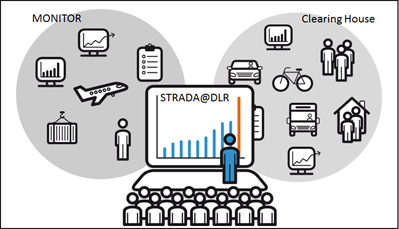
\includegraphics[width=0.8\textwidth]{strada-aproach.png}
  \caption{Aproximación del Proyecto \gls{strada} \cite{dublinstrada2}}
\end{figure}

Además de la mejora de la visualización de la información contenida, el portal ha de estar predispuesta a reforzarse y ampliarse con participación de otros institutos que aporten sus bases de datos sobre el ``Transporte y la Movilidad'' para continuar con el desarrollo del conocimiento en el \gls{dlr}.


\section{\IfLanguageName{english}{Scope}{Alcance}}
\label{section:alcance}

Este proyecto debe considerarse como un estudio piloto que establece las bases para la posible implementación usando otras fuentes de datos y permitiendo un mejor desarrollo en la gestión del conocimiento en el \gls{dlr}. Su finalidad es la mejora de la representación externa y la disposición de los datos del \gls{dlr} contribuyendo al fortalecimiento de la investigación sobre el ``\transmov''.\\

Para el público general como el especializado en los campos de política e industria se ofrecerán búsquedas avanzadas y optimizadas sobre los \glspl{metadato}, que son actualizados continuamente por los institutos involucrados. De igual forma, los usuarios deben ser atraídos por el grado de detalle y de calidad del contenido de la información proporcionada respecto a los  \glspl{metadato}. Por lo tanto, el \gls{dlr} jugará un papel importante como proveedor de servicios para la información sobre los datos incluso cuando por cuestiones de licencia estén restringidos para cierto grupos de usuarios.\\

Por este motivo, el objetivo principal de este proyecto es la creación de una nueva versión del \gls{framework} de búsqueda \gls{kf}, \gls{kf2}. Las  características más importantes del proyecto a mejorar se pueden desglosar en dos puntos principales; enriquecimiento de la visualización representando  estructuras y relaciones complejas de los datos y participación de nuevas fuentes de datos en el \gls{dlr} relacionadas con  el ``Transporte y la Movilidad''.\\
\subsection{Mejora de la visualización de estructuras y relaciones complejas de los datos}

La primera versión del proyecto \gls{kf} permite una búsqueda \gls{fulltext} sobre los datos de origen. Esta búsqueda está sólo centrada en el texto y, por lo tanto, muy limitada para los esquemas de \glspl{metadato} disponibles. Por ello, se deben diseñar e implementar para los usuarios finales unos sistemas de visualización avanzados que representen los esquemas de \glspl{metadato} dinámicos.\\

La finalidad de esta nueva visualización es la de representar las relaciones espaciales, temporales y contextuales entre los conjuntos y fuentes de datos y, por tanto, la generación de nuevos conocimientos y resultados que faciliten el proceso investigador y mejore la \gls{ux}.


\subsection{Participación de nuevas fuentes de datos en el DLR relacionadas con  el ``\transmov''}

Con el fin de aumentar el atractivo y valor del proyecto \gls{kf2} tanto dentro como fuera del \gls{dlr}, el sistema debe poder incorporar con relativa simpleza nuevas bases de datos adicionales relacionadas con el ``\transmov'' de institutos del \gls{dlr}.\\

Un claro ejemplo de estas posibilidades de mejora del conocimiento son el \gls{ts} y el \gls{fk}. Ambos poseen una base del conocimiento relacionada con el ``Transporte y la Movilidad'' y un declarado interés por contribuir a una fuente unificada de conocimiento conjunta.\\


\section{\IfLanguageName{english}{Document Structure}{Organización del
documento}} 
% \todo[inline]{Descripción de los contenidos de la presente memoria, así como del software entregado en soporte informático.}

Este documento explica el proceso de desarrollo de la aplicación \gls{kf2} y la aplicación para el portal \gls{strada}.\\

Empezando por la descripción de los objetivos iniciales y requisitos esenciales que deberá reunir dicho proyecto, 
se describe la planificación temporal del proyecto en un diagrama de \gls{gantt}, los costes estimados, estudio de los riesgos y la calidad del sistema.\\

A medida que se avance por el esta documentación, se irá explicando las fases del desarrollo del software; estudio del sistema actual y los requisitos y selección de la solución, análisis del sistema incluyendo gráficos \gls{uml} para los de casos de uso, diseño del sistema a implantar desglosado en módulos, explicación de la implementación y las pruebas realizadas.\\

Para finalizar, se incluyen los manuales necesarios para la implantación y explotación del \gls{software} y el manual para el usuario final. También se comentan las posibles mejoras o aplicaciones que pudieran considerarse en futuras versiones de este \gls{software}.